\documentclass[12pt]{article}
\usepackage{hyperref}
\usepackage[warn]{mathtext}
\usepackage[T2A]{fontenc}
\usepackage[utf8]{inputenc}
\usepackage[russian]{babel}
\usepackage{cite}
\usepackage{amsfonts}
\usepackage{lineno}
\usepackage{subfig}
\usepackage{graphicx}
\usepackage{xcolor}
\usepackage{bm}
\usepackage{graphicx}
\usepackage{amssymb}
\usepackage{hyperref}
\usepackage[left=2cm,right=2cm,top=2cm,bottom=2cm]{geometry}
\usepackage{indentfirst}
\DeclareSymbolFont{T2Aletters}{T2A}{cmr}{m}{it}

\DeclareGraphicsExtensions{.png,.jpg,.svg,.pdf}
\author{Карцев Вадим}
\title{Лабораторная работа 1.3

Эффект Рамзауэра}

\begin{document}

  \maketitle

  \textbf{Цель работы:} исследование энергетической зависимости вероятности
  рассеяния электронов атомами инертного газа, определение энергий электронов
  при которых наблюдается <<просветление>> инертного газа, оценка размера его
  внешней электронной оболочки.

  \textbf{Оборудование:} лампа-тиратрон, блок источников питания, осцилограф,
  вольтметр.

  \section{Краткое содержание}

    В данной лабораторной работе мы исследовали динамическим и статическим
    методом ВАХ тиратрона и получили значения для размера внешней атомной
    оболочки и определили газ, которым наполнен тиратрон. Этим газом оказался
    ксенон, а размер внешней электронной оболочки оказался равен примерно
    $151 пм$.

  \section{Теоретическая справка}

    Рассеяние электрона на атоме можно приближенно рассматривать как рассеяние
    частицы энергии $E$ на потенциальной яме длины $l$ и глубины $U_0$.
    Уравнение Шрёдингера имеет вид

    $$
      \Psi'' + k^2 \Psi = 0
    $$

    где $k_1$ вне ямы и $k_2$ внутри равны соответственно

    $$
      k^2 = k_1^2 = \frac{2 m E}{\hbar^2}
      \hspace{1cm}
      k^2 = k_2^2 = \frac{2 m \left(E + U_0\right)}{\hbar^2}
    $$

    В таком случае коэффициент прохождения равен

    $$
      D = \frac{16 k_1^2 k_2^2}{16 k_1^2 k_2^2 + 4 \left(k_1^2 - k_2^2\right)^2
      \sin^2 \left(k_2 l\right)}
    $$

    Легко заметить, что коэффициент прохождения имеет ряд максимумов и минимумов.
    Максимумы будут наблюдаться при соблюдении условия

    \begin{equation}
      \sqrt{\frac{2 m \left(E + U_0\right)}{\hbar^2}} l = n \pi, \hspace{0.3cm}
      n = 1, 2, 3, \ldots
      \label{eq:maximums}
    \end{equation}

    Качественно эффект Рамзауэра можно объяснить, рассмотрев интерференцию
    прошедшей и дважды отразившейся от оболочки волн де Бройля. Длины волн вне и
    внутри атома

    $$
      \lambda = \frac{h}{\sqrt{2 m E}}, \hspace{0.3cm}
      \lambda_1 = \frac{h}{\sqrt{2 m \left(E + U_0\right)}}
    $$

    Тогда условия на первые интерференционные максимумы и минимумы выглядят
    следующим образом

    \begin{equation}
      2 l = \frac{h}{\sqrt{2 m \left(E_1 + U_0\right)}}
      \hspace{1cm}
      2 l = \frac{3}{2} \frac{h}{\sqrt{2 m \left(E_2 + U_0\right)}}
      \label{eq:max_min_gain_weakening}
    \end{equation}

    Так же можно исключить из этих соотношений глубину потенциальной ямы

    \begin{equation}
      l = \frac{h \sqrt{5}}{\sqrt{32 m \left( E_2 - E_1 \right)}}
      \label{eq:atom_size}
    \end{equation}

    При этом глубина ямы будет равна

    \begin{equation}
      U_0 = \frac{4}{5} E_2 - \frac{9}{5} E_1
      \label{eq:potential_pit_depth}
    \end{equation}

  \section{Обработка результатов динамического режима}

  \begin{figure}[h!]
    \center{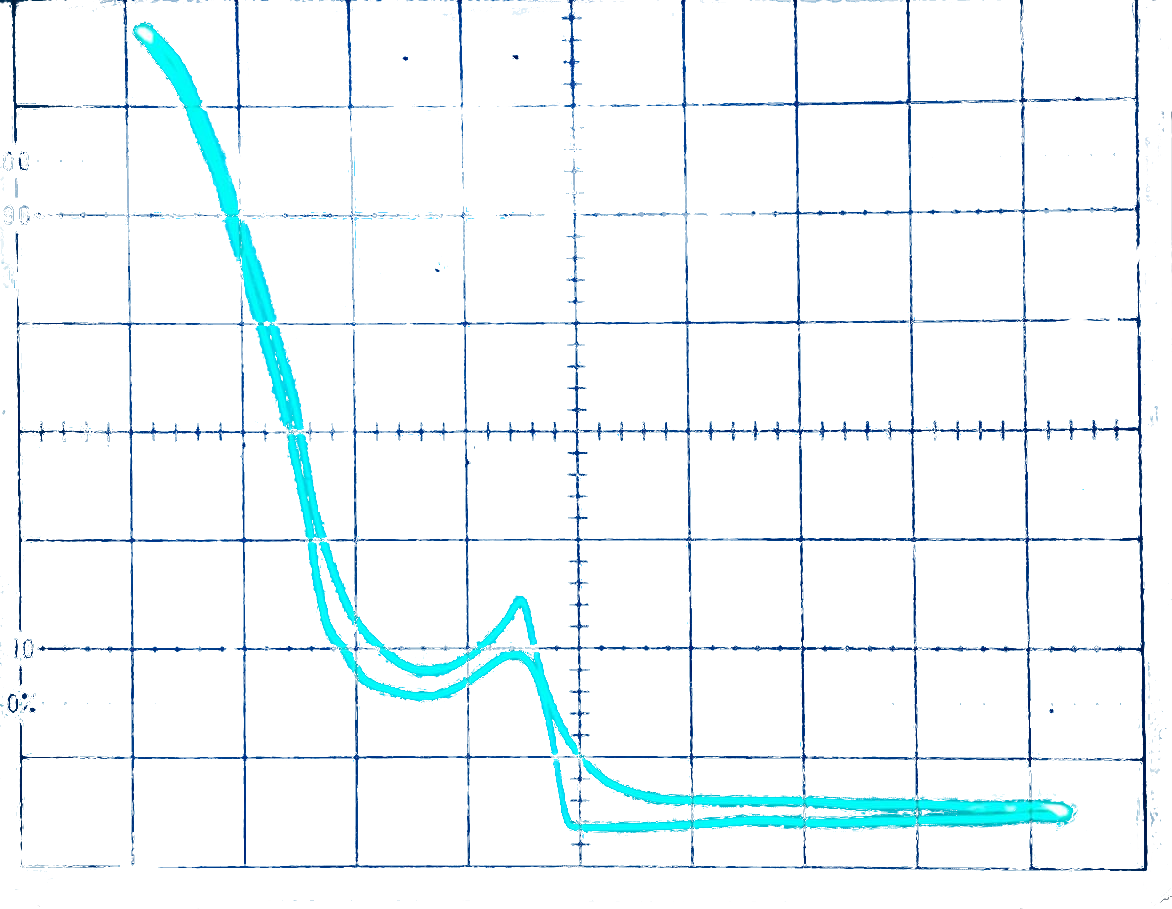
\includegraphics[width = 0.49\linewidth]{oscillogram.png}}\\
    Рис 1. Осциллограмма
    \label{fig:oscillograme}
  \end{figure}

    \subsection{Рассчет размера электронной оболочки атома}

      В обоих случаях мы получили значения максимума $E_1 = 2,5$ эВ и
      минимума $E_2 = 7$ эВ. Подставим измеренные значения в формулы
      \ref{eq:max_min_gain_weakening}.

      $$
        2 l = \frac{6,63 \cdot 10^{-34}}{\sqrt{2 \cdot 9,11 \cdot 10^{-31} \cdot
        \left( 2,5 + 2,5 \right) \cdot 6,24 \cdot 10^{-19}}} \approx 278 пм;
        \hspace{1cm} l = \frac{278}{2} \approx 139 пм
      $$
      $$
        2 l = \frac{3}{2} \frac{6,63 \cdot 10^{-34}}{\sqrt{2 \cdot 9,11 \cdot
        10^{-31} \cdot \left( 7 + 2,5 \right) \cdot 6,24 \cdot 10^{-19}}}
        \approx 302 пм; \hspace{1cm} l = \frac{302}{2} \approx 151 пм
      $$

      Точно так же подставим полученные данные в формулу \ref{eq:atom_size}.

      $$
        l = \frac{6,63 \cdot 10^{-34} \cdot \sqrt{5}}{\sqrt{32 \cdot 9,11 \cdot
        10^{-31} \cdot \left( 7 - 2,5 \right) \cdot 6,24 \cdot 10^{-19}}}
        \approx 164 пм
      $$

      Таким образом мы получили, что размер электронной оболчки атома $l
      \approx 151 пм$

    \subsection{Оценка глубины потенциальной ямы}

      Подставим в уравнение \ref{eq:potential_pit_depth} измеренные значения.

      $$
        U_0 = \frac{4}{5} \cdot 7 - \frac{9}{5} \cdot 2.5 = 1,1 В
      $$

    \subsection{Оценка потенциала ионизации}

      В динамическом методе мы получили напряжение пробоя $U_п \approx 12$ В.
      Таким образом мы можем сказать, что тиратрон наполнен \textbf{ксеноном},
      для которого ионизационный потенциал $U_{п_{Xe}} = 12,1$ эВ

  \section{Обработка результатов статического режима}

    \subsection{Построение графиков зависимости $I_а = f(V_с)$}

      \begin{figure}[h!]
        \begin{minipage}[h]{0.49\linewidth}
            \center{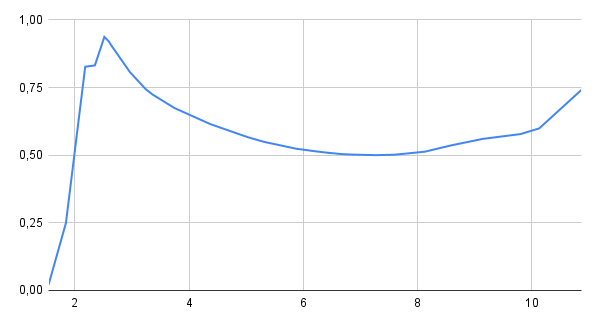
\includegraphics[width = \linewidth]{plot3.07.png}}\\
            Рис 2. График для $V_н = 3,07$ В
        \end{minipage}
        \begin{minipage}[h]{0.49\linewidth}
            \center{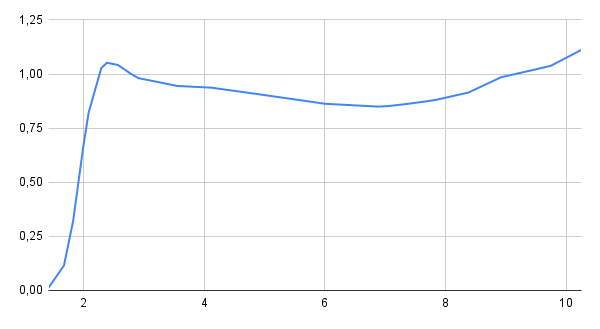
\includegraphics[width = \linewidth]{plot3.32.png}}\\
            Рис 3. График для $V_н = 3,32$ В
        \end{minipage}
        \label{fig:static_plots}
      \end{figure}

      Графики построены по таблицам данных, приведённым в разделе
      <<Дополнительные данные>> на стр. \pageref{table:static_method}.

      Из графиков видно что для $V_н = 3,07$ В максимум достигается при
      $V_1 = 2,515$ В а минимум при $V_2 = 7,279$ В.
      Для $V_н = 3,32$ В эти значения $V_1 = 2,39$ В и $V_2 = 6,889$ В.

    \subsection{Вычисление размера атома}

      Подставим значения для $V_н = 3,07$ В в формулы
      \ref{eq:max_min_gain_weakening} и \ref{eq:atom_size}.

      $$
        2 l = \frac{6,63 \cdot 10^{-34}}{\sqrt{2 \cdot 9,11 \cdot 10^{-31} \cdot
        \left( 2,515 + 2,5 \right) \cdot 6,24 \cdot 10^{-19}}} \approx 277 пм;
        \hspace{1cm} l = \frac{277}{2} \approx 139 пм
      $$

      $$
        2 l = \frac{3}{2} \frac{6,63 \cdot 10^{-34}}{\sqrt{2 \cdot 9,11 \cdot
        10^{-31} \cdot \left( 7,279 + 2,5 \right) \cdot 6,24 \cdot 10^{-19}}}
        \approx 298 пм; \hspace{1cm} l = \frac{298}{2} \approx 149 пм
      $$

      $$
        l = \frac{6,63 \cdot 10^{-34} \cdot \sqrt{5}}{\sqrt{32 \cdot 9,11 \cdot
        10^{-31} \cdot \left( 7,279 - 2,515 \right) \cdot 6,24 \cdot 10^{-19}}}
        \approx 159 пм
      $$

      Таким же образом поступим и с данными для $V_н = 3,32$ В

      $$
        2 l = \frac{6,63 \cdot 10^{-34}}{\sqrt{2 \cdot 9,11 \cdot 10^{-31} \cdot
        \left( 2,39 + 2,5 \right) \cdot 6,24 \cdot 10^{-19}}} \approx 281 пм;
        \hspace{1cm} l = \frac{281}{2} \approx 140 пм
      $$

      $$
        2 l = \frac{3}{2} \frac{6,63 \cdot 10^{-34}}{\sqrt{2 \cdot 9,11 \cdot
        10^{-31} \cdot \left( 6,889 + 2,5 \right) \cdot 6,24 \cdot 10^{-19}}}
        \approx 304 пм; \hspace{1cm} l = \frac{304}{2} \approx 152 пм
      $$

      $$
        l = \frac{6,63 \cdot 10^{-34} \cdot \sqrt{5}}{\sqrt{32 \cdot 9,11 \cdot
        10^{-31} \cdot \left( 6,889 - 2,39 \right) \cdot 6,24 \cdot 10^{-19}}}
        \approx 164 пм
      $$

      Усредним размер электронной оболчки атома, полученный для разных
      напряжений накала. Тогда искомый размер $l \approx 151 пм$.

    \subsection{Оценка глубины потенциальной ямы}

      Рассчитаем глубину потенцальной ямы для $V_н = 3,07$ В:

      $$
        U_0 = \frac{4}{5} \cdot 7,279 - \frac{9}{5} \cdot 2,515 = 1,2962 В
      $$

      и для $V_н = 3,32$ В:

      $$
        U_0 = \frac{4}{5} \cdot 6,889 - \frac{9}{5} \cdot 2,39 = 1,2092 В
      $$

  \section{Теоретический рассчет напряжений с максимальным усилением}

    $$
      k_2 l = \sqrt{\frac{2 m \left( E_n + U_0 \right)}{\hbar^2}} l = \pi n
      \Rightarrow
      E_n = \frac{\left(\frac{\pi n \hbar}{l}\right)^2}{2 m} - U_0 =
      \frac{\pi^2 n^2 \hbar^2}{2 m l^2} - U_0
    $$

    Выразим $l$ из исходного выражения и подставим его в формулу.

    $$
      l = \frac{\pi \hbar n}{\sqrt{2 m \left( E_n + U_0 \right)}} =
      \frac{\pi \hbar}{\sqrt{2 m \left( E_1 + U_0 \right)}}
    $$

    $$
      E_n = f(E_1, n) = \frac{\pi^2 n^2 \hbar^2}{2 m
      \frac{\pi^2 \hbar^2}{2 m \left( E_1 + U_0 \right)}} - U_0 =
      \underbrace{\left( E_1 + U_0 \right) n^2 -
      U_0}_{\mbox{\scriptsize{Искомая зависимость}}}
    $$

    По полученой формуле рассчитаем напряжения на которых наблюдаются максимумы
    2-го и 3-го порядка, приняв $E_1 = 2,515 В$, $U_0 = 3,07 В$.\\

    \begin{tabular}{ | l | c | c | c | }
      \hline
      Порядок максимума & $1$ & $2$ & $3$ \\ \hline
      Напряжение максимума & $2,52В$ & $19,27В$ & $47,20В$ \\
      \hline
    \end{tabular}

    \section{Рассчет вероятности рассеяния электронов}

      По данным можно построить график зависимости вероятности рассеяния с
      точностью до константы \\

      \begin{figure}[h!]
        \center{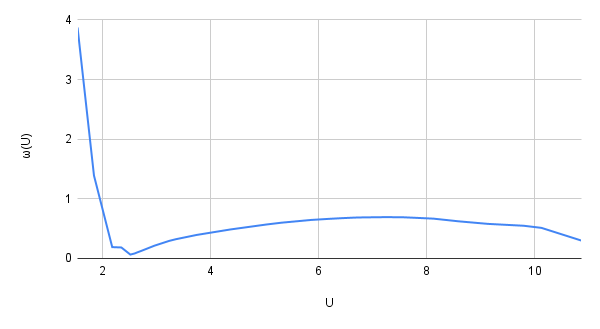
\includegraphics[width = 0.6\linewidth]{scattering_probability.png}}\\
        Рис 4. Зависимость вероятности рассеивания от энергии электронов
        \label{fig:oscillograme}
      \end{figure}

    \section{Вывод}
      В ходе работы была статическим и динамическим методом исследована ВАХ
      тиратрона, в обоих случаях соответствующая теоретической, получено
      значение размера внешней оболочки атома инертного газа и потенциал его
      ионизации, по которому было определено, что это ксенон.

    \newpage
    \section{Дополнительные данные}

      \begin{figure}[h!]
        \begin{minipage}[h]{0.49\linewidth}
          \center{$V_н = 3,07 В$}

          \begin{tabular}{ | c | c | c | c | }
            \hline
            $N$ & $V_c$ & $V_I$ & $I$ \\ \hline
            1 & 1,538 & 2,08 & 0,0208 \\
            2 & 1,842 & 24,9 & 0,249 \\
            3 & 2,18 & 82,7 & 0,827 \\
            4 & 2,349 & 83,18 & 0,8318 \\
            5 & 2,515 & 93,72 & 0,9372 \\
            6 & 2,595 & 92 & 0,92 \\
            7 & 2,636 & 90,59 & 0,9059 \\
            8 & 2,722 & 87,98 & 0,8798 \\
            9 & 2,961 & 80,75 & 0,8075 \\
            10 & 3,234 & 74,5 & 0,745 \\
            11 & 3,358 & 72,43 & 0,7243 \\
            12 & 3,742 & 67,43 & 0,6743 \\
            13 & 4,37 & 61,48 & 0,6148 \\
            14 & 5,029 & 56,63 & 0,5663 \\
            15 & 5,314 & 54,9 & 0,549 \\
            16 & 5,863 & 52,43 & 0,5243 \\
            17 & 6,185 & 51,5 & 0,515 \\
            18 & 6,422 & 50,91 & 0,5091 \\
            19 & 6,668 & 50,4 & 0,504 \\
            20 & 6,816 & 50,25 & 0,5025 \\
            21 & 7,14 & 50,07 & 0,5007 \\
            22 & 7,279 & 50,02 & 0,5002 \\
            23 & 7,577 & 50,16 & 0,5016 \\
            24 & 7,786 & 50,57 & 0,5057 \\
            25 & 8,127 & 51,3 & 0,513 \\
            26 & 8,589 & 53,64 & 0,5364 \\
            27 & 9,135 & 56,01 & 0,5601 \\
            28 & 9,799 & 57,8 & 0,578 \\
            29 & 10,126 & 59,89 & 0,5989 \\
            30 & 10,866 & 74,13 & 0,7413 \\
            \hline
          \end{tabular}

        \end{minipage}
        \begin{minipage}[h]{0.49\linewidth}
          \center{$V_н = 3,32 В$}

          \begin{tabular}{ | c | c | c | c | }
            \hline
            $N$ & $V_c$ & $V_i$ & $I$ \\ \hline
            1 & 1,422 & 1,25 & 0,0125 \\
            2 & 1,677 & 11,5 & 0,115 \\
            3 & 1,83 & 32,2 & 0,322 \\
            4 & 1,996 & 66,2 & 0,662 \\
            5 & 2,086 & 82,15 & 0,8215 \\
            6 & 2,295 & 102,74 & 1,0274 \\
            7 & 2,39 & 105,21 & 1,0521 \\
            8 & 2,569 & 104,19 & 1,0419 \\
            9 & 2,626 & 103,13 & 1,0313 \\
            10 & 2,795 & 99,92 & 0,9992 \\
            11 & 2,907 & 98,13 & 0,9813 \\
            12 & 3,555 & 94,48 & 0,9448 \\
            13 & 4,117 & 93,7 & 0,937 \\
            14 & 4,905 & 90,65 & 0,9065 \\
            15 & 6,005 & 86,25 & 0,8625 \\
            16 & 6,889 & 84,94 & 0,8494 \\
            17 & 7,044 & 85,17 & 0,8517 \\
            18 & 7,396 & 86,3 & 0,863 \\
            19 & 7,683 & 87,4 & 0,874 \\
            20 & 7,854 & 88,15 & 0,8815 \\
            21 & 8,377 & 91,45 & 0,9145 \\
            22 & 8,916 & 98,5 & 0,985 \\
            23 & 9,533 & 102,41 & 1,0241 \\
            24 & 9,743 & 103,82 & 1,0382 \\
            25 & 10,249 & 111,17 & 1,1117 \\
            \hline
          \end{tabular}

          \vspace{2.52cm}
        \end{minipage}
        \label{table:static_method}
      \end{figure}

\end{document}
